\documentclass[aspectratio=169]{beamer}
\usetheme{metropolis}
\metroset{block=fill}

\usepackage{newpxtext}
\usepackage{newpxmath}

\usepackage{graphicx}
\usepackage{physics}
\usepackage{ragged2e}

\usepackage{pgfplots}
\pgfplotsset{width=\textwidth, height=0.494427\textwidth}


\usepackage{tikz}
\usepackage{mathtools}
\usetikzlibrary{positioning, shapes.geometric, arrows, arrows.meta}

\usefonttheme{serif}

\title{Optically-Active Media}
\subtitle{The QuEST for fast models}
\date{December 20, 2017}
\author{Connor Glosser}
\institute{Michigan State University}

\begin{document}

\maketitle

\section{About me}

\begin{frame}
  \vspace{0.7cm}
  \begin{columns}[c]
    \column{0.5\textwidth}
      \hfill 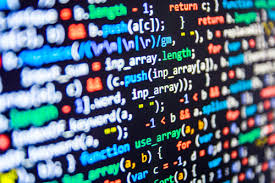
\includegraphics[width=0.8\textwidth]{figures/coding.jpg} \\ \vspace{0.6cm}
      \hfill 
\includegraphics[width=0.8\textwidth]{figures/collaboration.jpg}

    \column{0.5\textwidth}
      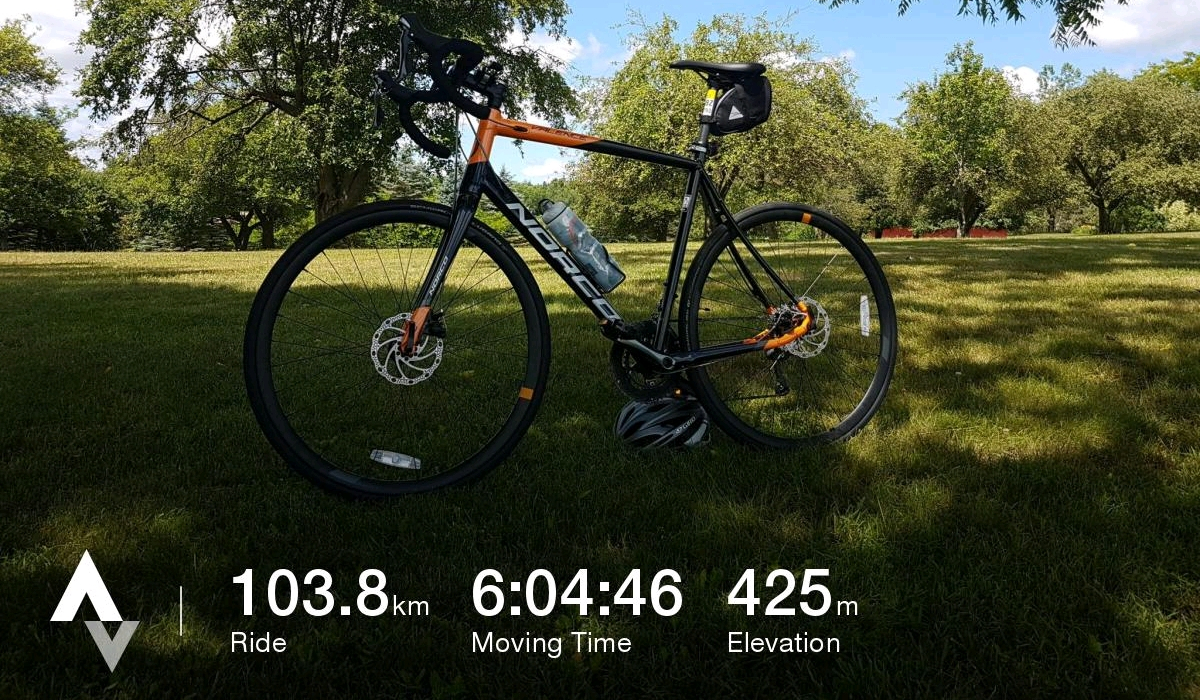
\includegraphics[width=0.8\textwidth]{figures/strava_cropped.jpg} \vspace{0.6cm}
      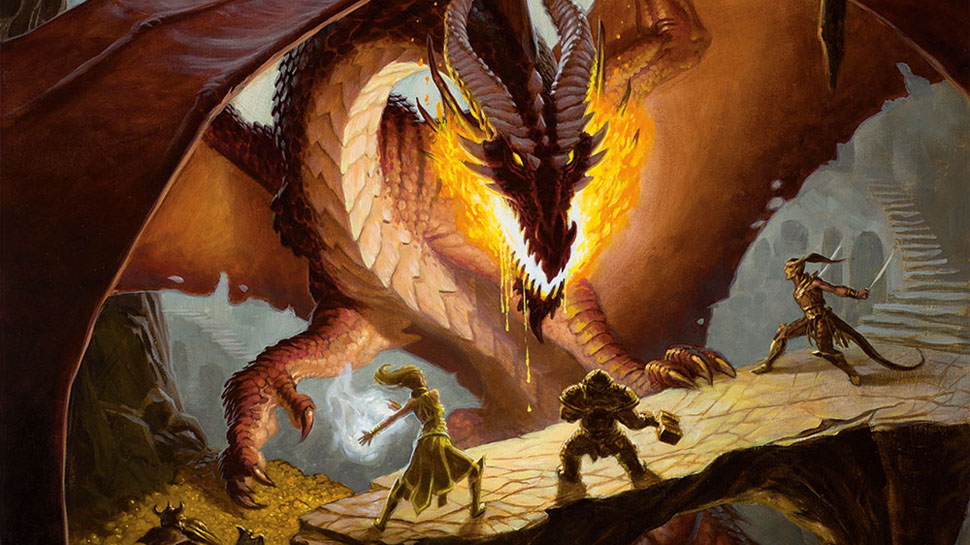
\includegraphics[width=0.8\textwidth]{figures/dnd.jpg}
  \end{columns}
\end{frame}

\begin{frame}{Things I've worked on}
  \begin{itemize}
    \item Radiation models (particularly quantum optics: QuEST)
      \begin{itemize}
        \item Rank-deficient fast methods, performance optimization, tree codes, FFTs, GPUs
      \end{itemize}
    \item Hydrocarbon deposition molecular dynamics (REBO)
    \item Nanostructure inverse problem/structure reconstruction (Tribond)
    \item Computational physics education
      \begin{itemize}
        \item \textbf{I}nternational \textbf{C}ourse in \textbf{C}omputational \textbf{P}hysics
        \item Course development, teaching assistantships
        \item Introductory workshops (highschool and college level)
      \end{itemize}
  \end{itemize}
\end{frame}

\begin{frame}
  \begin{center}
    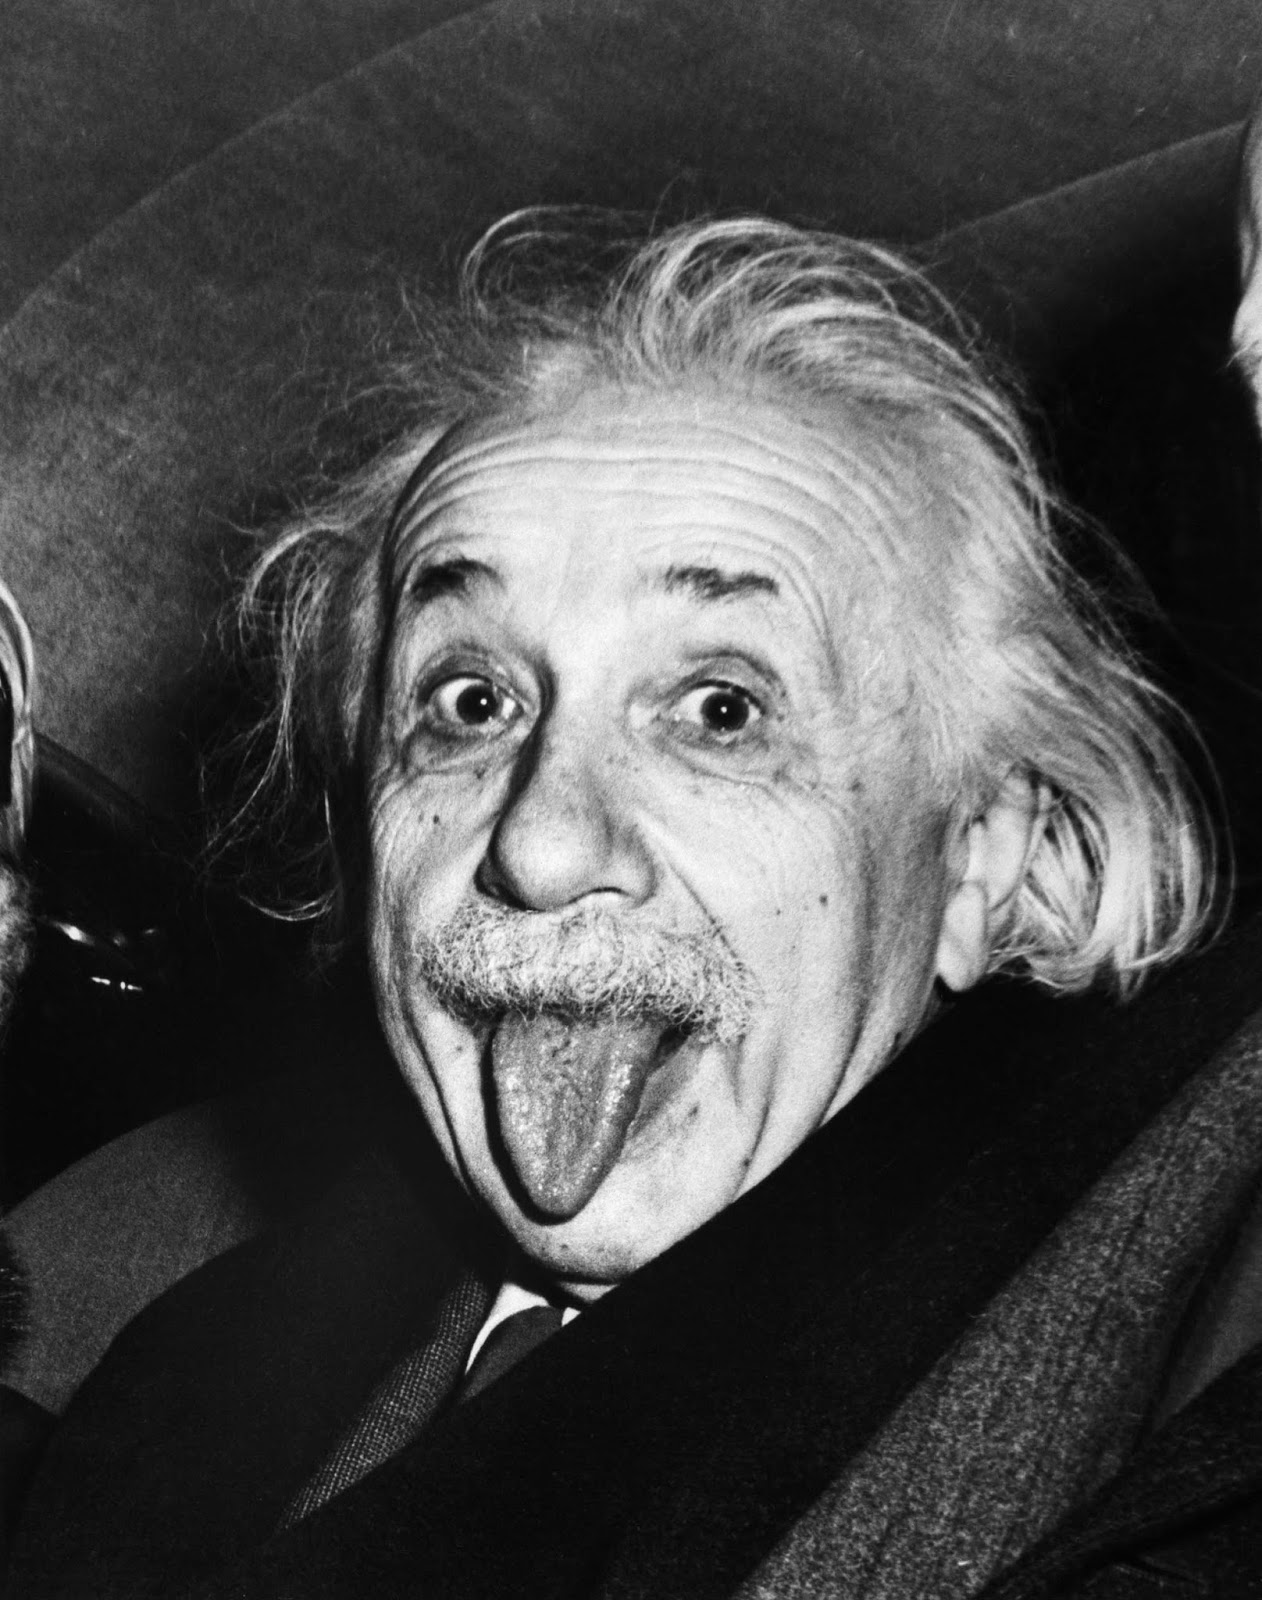
\includegraphics[width=0.3\textwidth]{figures/einstein_tongue.jpg}
    \hspace{0.1cm}
    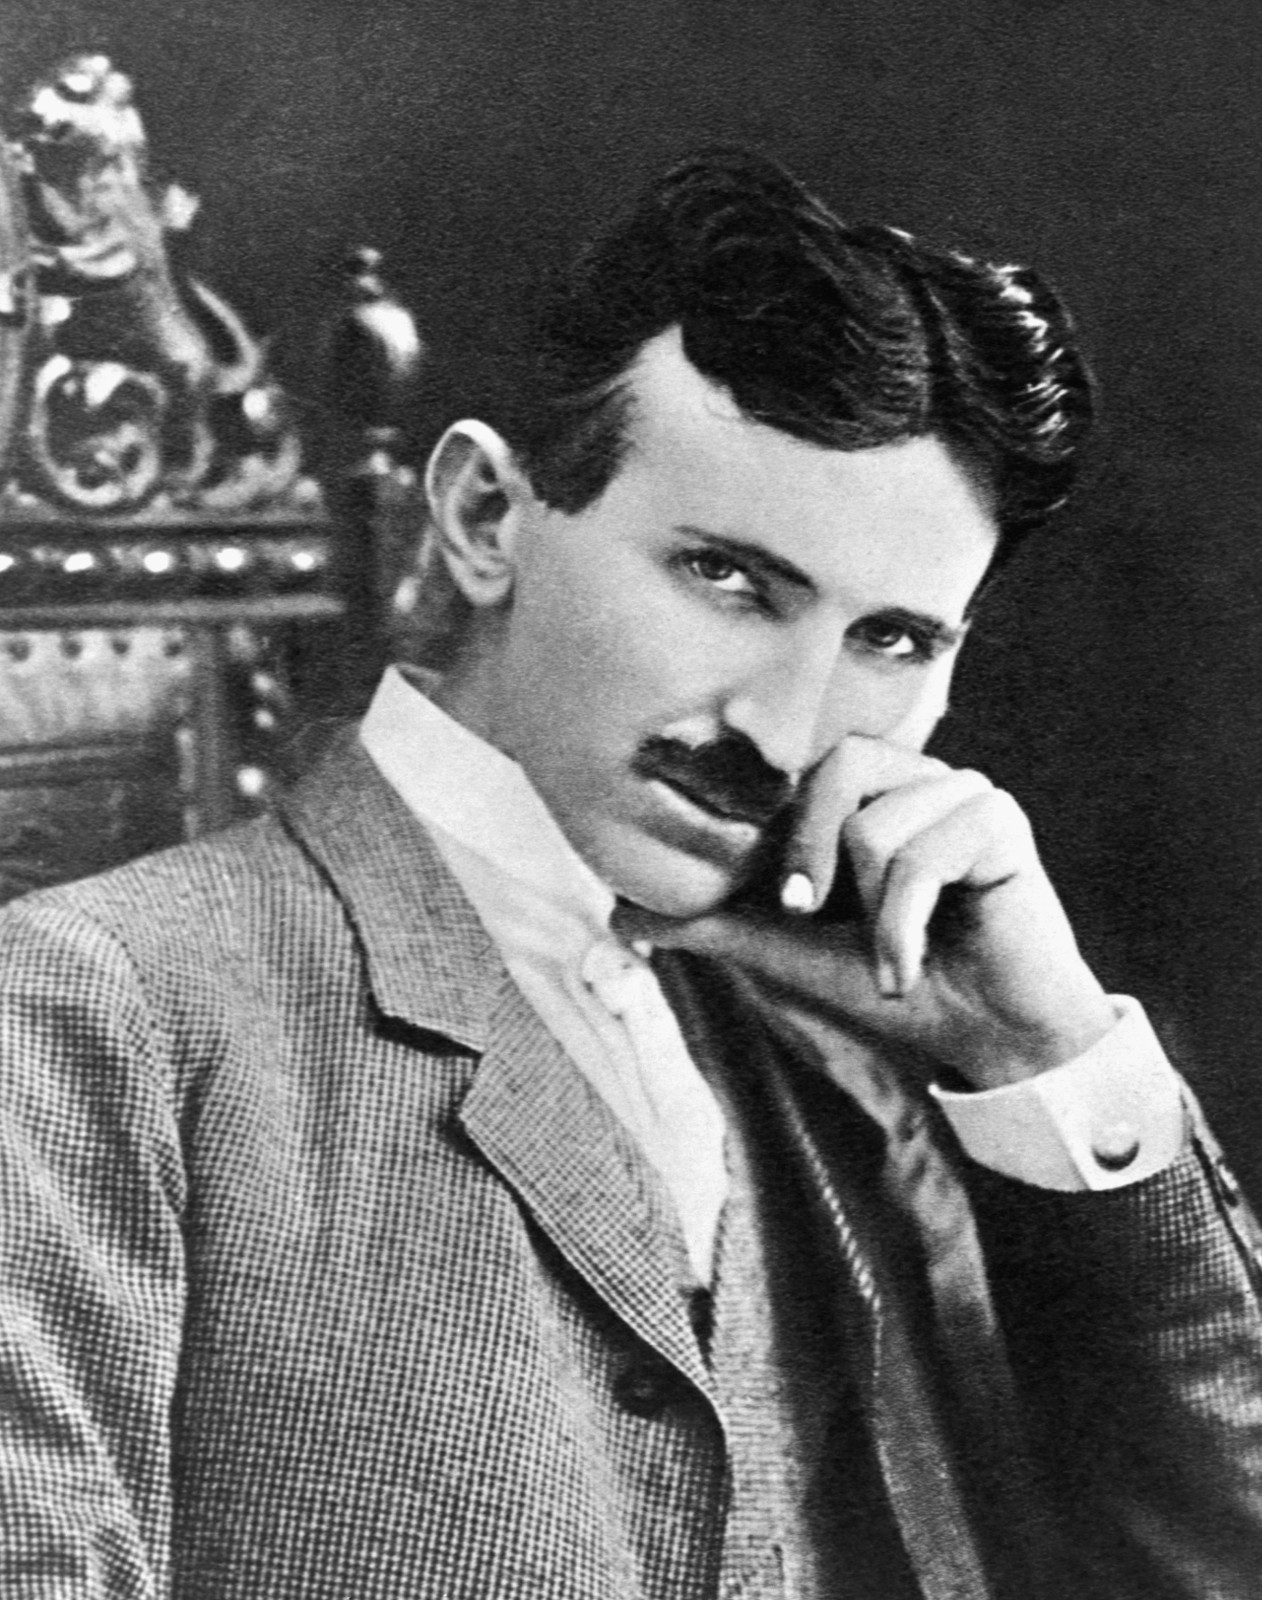
\includegraphics[width=0.3\textwidth]{figures/tesla_chair.jpg}
  \end{center}
\end{frame}

\section{Designing an algorithm}

\subsection{Quantum}

\begin{frame}
  \vspace{-1cm}
  \begin{columns}
    \begin{column}{0.25\textwidth}
      \begin{center}
        Photovoltaics
      \end{center}
    \end{column}

    \begin{column}{0.25\textwidth}
      \begin{center}
        Next-gen displays
      \end{center}
    \end{column}

    \begin{column}{0.25\textwidth}
      \begin{center}
        Biological contrast
      \end{center}
    \end{column}

    \begin{column}{0.25\textwidth}
      \begin{center}
        Quantum computing
      \end{center}
    \end{column}

  \end{columns}

  \begin{columns}
    \begin{column}{0.25\textwidth}
      \begin{figure}
        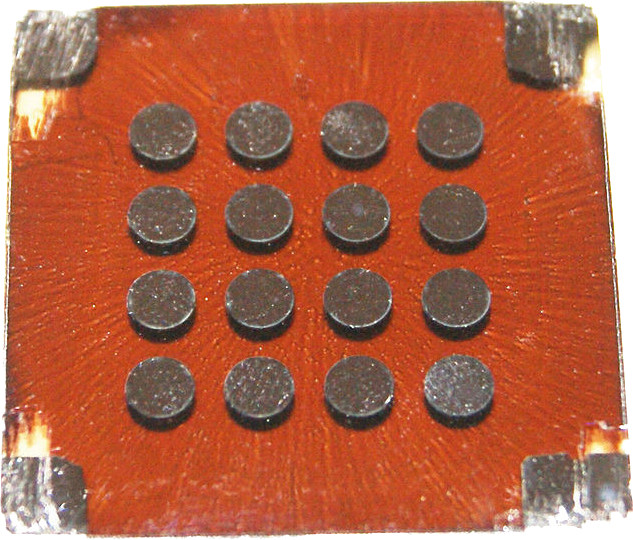
\includegraphics[width=\textwidth]{figures/devices/quantum_dot_solar_cell.jpg}
      \end{figure}
    \end{column}

    \begin{column}{0.25\textwidth}
      \begin{figure}
        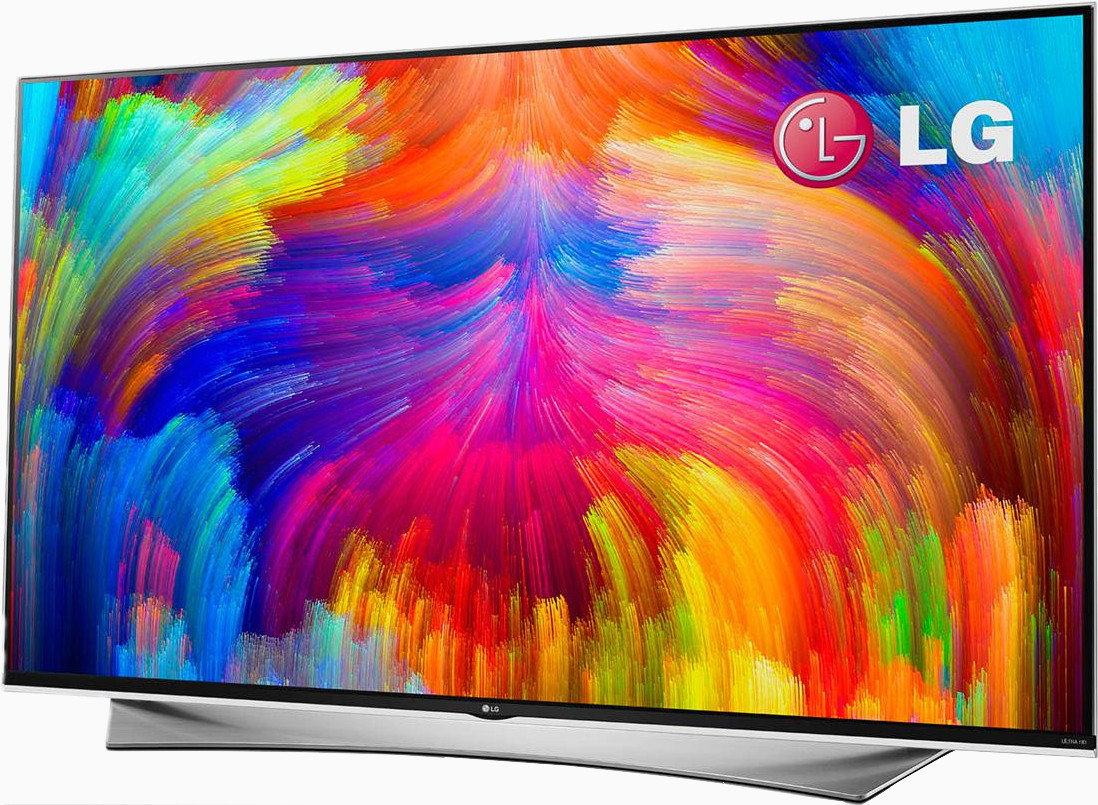
\includegraphics[width=\textwidth]{figures/devices/quantum_dot_tv.jpg}
      \end{figure}
    \end{column}

    \begin{column}{0.25\textwidth}
      \begin{figure}
        \vspace{-1.2em}
        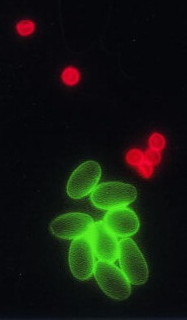
\includegraphics[width=\textwidth, height=0.4\textheight]{figures/devices/contrast.jpg}
      \end{figure}
    \end{column}

    \begin{column}{0.25\textwidth}
      \begin{figure}
        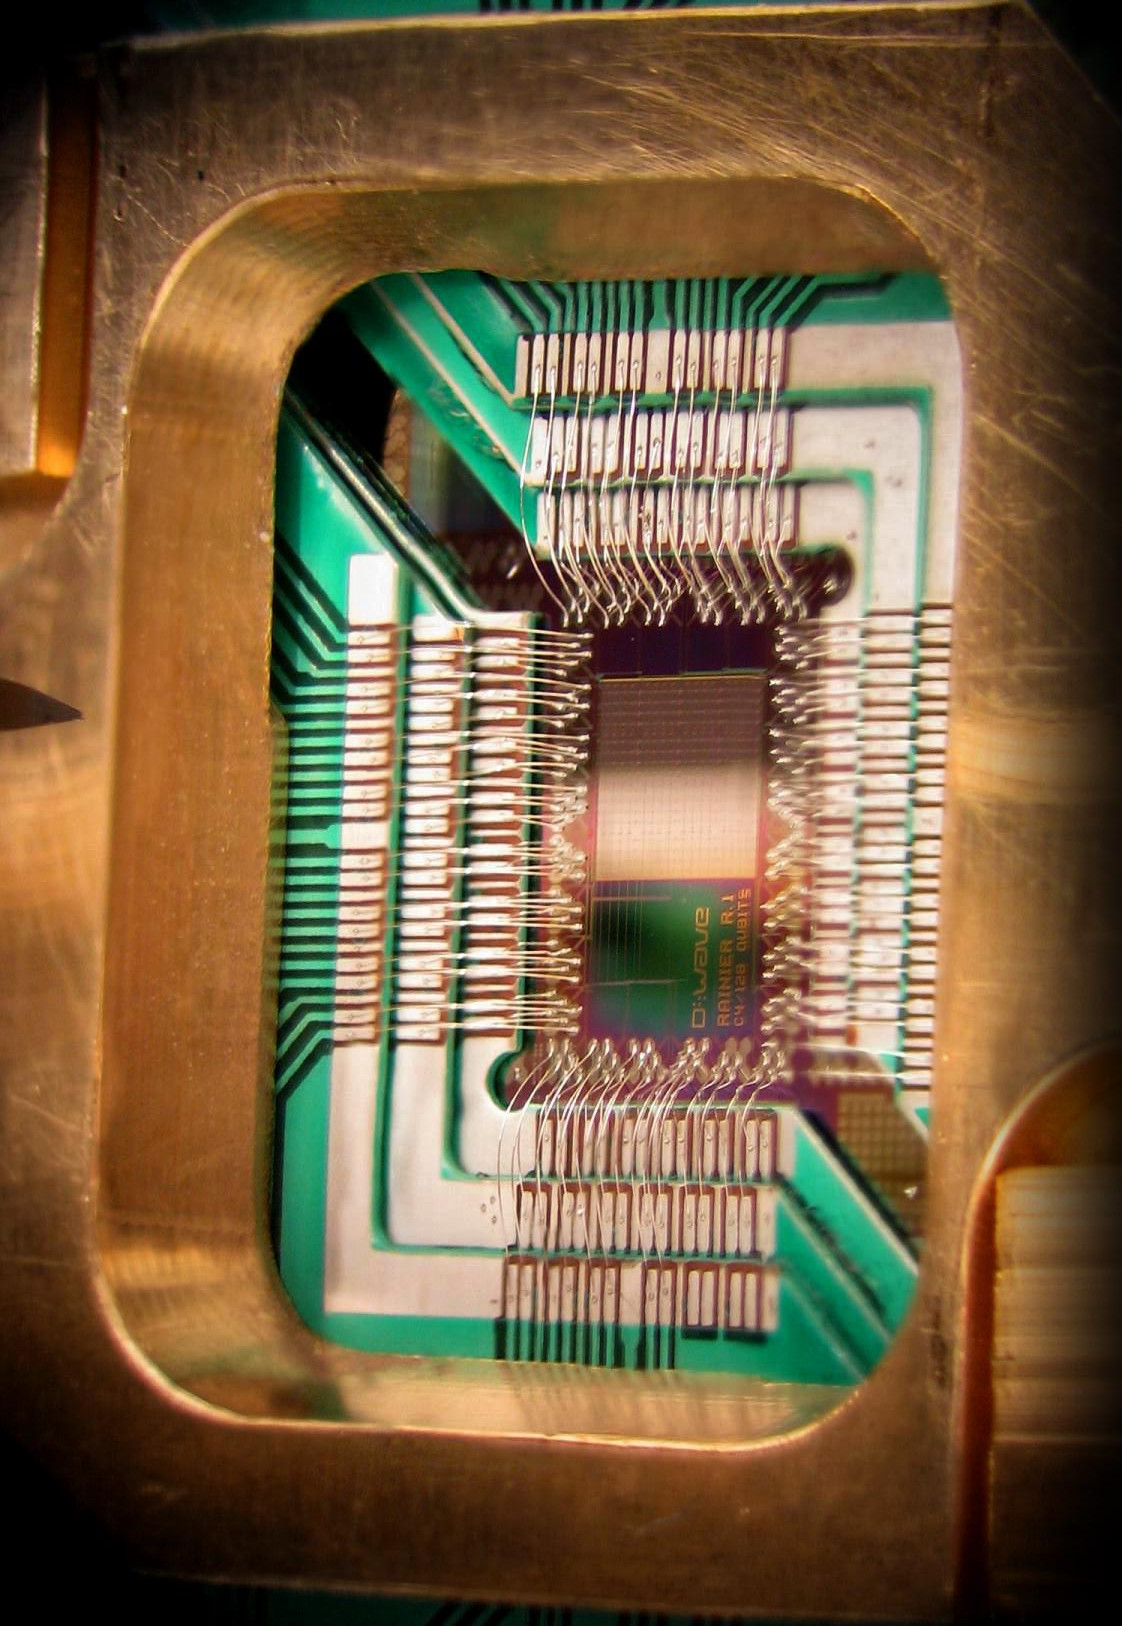
\includegraphics[width=\textwidth]{figures/devices/quantum_computer.jpg}
      \end{figure}
    \end{column}
  \end{columns}
\end{frame}

\begin{frame}{Simulated quantum dot = two-level system}
  \begin{columns}[c]
    \column{0.3\textwidth}
      \centering
      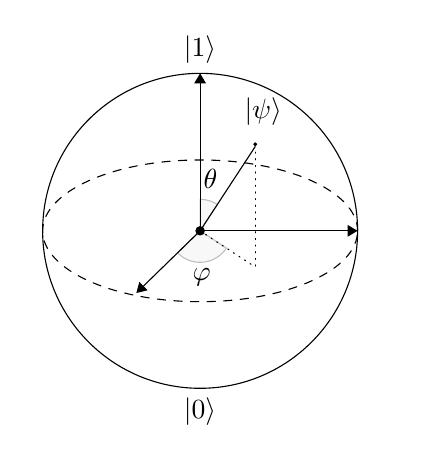
\begin{tikzpicture}[line cap=round, line join=round, >=Triangle]
  \clip(-2.19,-2.49) rectangle (2.66,2.58);
  \draw [shift={(0,0)}, lightgray, fill, fill opacity=0.1] (0,0) -- (56.7:0.4) arc (56.7:90.:0.4) -- cycle;
  \draw [shift={(0,0)}, lightgray, fill, fill opacity=0.1] (0,0) -- (-135.7:0.4) arc (-135.7:-33.2:0.4) -- cycle;
  \draw(0,0) circle (2cm);
  \draw [rotate around={0.:(0.,0.)},dash pattern=on 3pt off 3pt] (0,0) ellipse (2cm and 0.9cm);
  \draw (0,0)-- (0.70,1.07);
  \draw [->] (0,0) -- (0,2);
  \draw [->] (0,0) -- (-0.81,-0.79);
  \draw [->] (0,0) -- (2,0);
  \draw [dotted] (0.7,1)-- (0.7,-0.46);
  \draw [dotted] (0,0)-- (0.7,-0.46);
  \draw (-0.22,-0.35) node[anchor=north west] {$\varphi$};
  \draw (-0.08,0.9) node[anchor=north west] {$\theta$};
  %\draw (-1.01,-0.72) node[anchor=north west] {$\vu{x}$};
  %\draw (2.07,0.3) node[anchor=north west] {$\vu{y}$};
  \draw (0,-2) node[anchor=north] {$\ket{0}$};
  \draw (0,2.6) node[anchor=north] {$\ket{1}$};
  \draw (0.44, 1.815) node[anchor=north west] {$\ket{\psi}$};
  \scriptsize
  \draw [fill] (0,0) circle (1.5pt);
  \draw [fill] (0.7,1.1) circle (0.5pt);
\end{tikzpicture}


    \column{0.7\textwidth}
      \begin{itemize}
        \item ``Artifical atoms'' (tuneable spectrum)
        \item Two-level quantum state: $\ket*{\psi} = \alpha \ket{0} + \beta \ket{1}$
        \item $\Delta \mathcal{E} \sim$ optical frequencies; radius $\ll \lambda$
        \item Dynamical absorbtion and emission
      \end{itemize}

      \begin{block}{Liouville equation}
        \begin{equation*}
          \dv{\hat{\rho}}{t} = \commutator{\hat{\mathcal{H}}}{\hat{\rho}} - \hat{\mathcal{D}}\qty[\hat{\rho}]; \quad \hat{\rho} = \dyad{\psi}{\psi}
        \end{equation*}
        \hfill {\tiny(mixed-state analogue of Schr\"odinger equation)}
      \end{block}
  \end{columns}
\end{frame}

\begin{frame}
  \begin{columns}
    \column{0.5\textwidth}
      \begin{equation*}
        \hat{\mathcal{H}} = \mqty(0 & \vb{d} \cdot \vb{E}(t) \\ \qty\big(\vb{d} \cdot \vb{E}(t))^* & \hbar \omega_0)
      \end{equation*}
      \begin{itemize}
        \item Unperterbed $\hat{\mathcal{H}}$ diagonalized by $\ket{0}, \ket{1}$.
        \item Couples evolution to $\vb{E}$-field
        \item $\vb{d} = \matrixelement{0}{e \hat{\vb{r}}}{1}$
      \end{itemize}

    \column{0.5\textwidth}
      \begin{equation*}
        \hat{\mathcal{D}}\qty[\hat{\rho}] = \mqty((\rho_{00} - 1)/T_1 & \rho_{01}/T_2 \\ \rho_{10}/T_2 & \rho_{11}/T_1)
      \end{equation*}
      \begin{itemize}
        \item Phenomenological dissipator
        \item Returns $\hat{\rho}$ to ground state with characteristic $T_1, T_2$ times
      \end{itemize}
  \end{columns}
\end{frame}

\subsection{Electromagnetics}

\begin{frame}{Lightning review of (linear) Green's functions}
  To solve the following differential equation for $a(x)$ \ldots
  \begin{equation*}
    \hat{\mathcal{L}}\qty[a(x)] = b(x)
  \end{equation*}
  \ldots it's far easier to \emph{first} find the Green's function,
  \begin{equation*}
    \hat{\mathcal{L}}\qty[g(x, x')] = \delta(x - x').
  \end{equation*}
  Then,
  \begin{align*}
    \hat{\mathcal{L}}\qty[a(x)] &= \int \delta(x - x') b(x') \dd{x'} \\
                                &= \int \hat{\mathcal{L}}\qty[g(x, x')] b(x') \dd{x'} \\
                   \Aboxed{a(x) &= \int g(x, x') b(x') \dd{x'}}
  \end{align*}
\end{frame}

\begin{frame}
  \begin{block}{Laplace equation}
    \begin{equation*}
      \laplacian g(\vb{r}, \vb{r}') = -4 \pi \delta(\vb{r} - \vb{r}') \implies g(\vb{r}, \vb{r}') = \frac{1}{\abs{\vb{r} - \vb{r}'}}
    \end{equation*}
  \end{block}

  \begin{block}{Wave equation}
    \begin{equation*}
      \qty(\laplacian - \frac{1}{c^2}\pdv[2]{t}) g^{(4)} = -4 \pi \delta^{(4)} \implies g(\vb{r}, t; \vb{r}', t') = \frac{\delta(\vb{r} - \vb{r}')}{\abs{\vb{r} - \vb{r}'}} \delta\qty(t - t' - \frac{\abs{\vb{r} - \vb{r}'}}{c})
    \end{equation*}
  \end{block}
\end{frame}

\begin{frame}{Maxwell's equations}
  %\begin{alignat*}{2}
    %\div \vb{E} &= 4 \pi k_1 \rho  \qquad &  \curl \vb{B} &= 4 \pi k_2 \alpha \vb{J} + \frac{k_2 \alpha}{k_1} \pdv{\vb{E}}{t} \\
    %\curl \vb{E} &= -k_3 \pdv{\vb{B}}{t} \qquad & \div \vb{B} &= 0
  %\end{alignat*}
  \begin{align*}
    \scalebox{2}{$\div \vb{E}$} & \scalebox{2}{$\; = 4 \pi k_1 \rho$} &  \scalebox{1.5}{\text{Gauss}}\\
    \scalebox{2}{$\curl \vb{B}$} & \scalebox{2}{$\; = 4 \pi k_2 \alpha \vb{J} + \frac{k_2 \alpha}{k_1} \pdv{\vb{E}}{t}$} & \scalebox{1.5}{\text{Amp\`ere}} \\
    \scalebox{2}{$\div \vb{B}$} & \scalebox{2}{$\; = 0$} & \scalebox{1.5}{\text{Gauss}} \\
    \scalebox{2}{$\curl \vb{E}$} & \scalebox{2}{$\; = -k_3 \pdv{\vb{B}}{t}$} & \scalebox{1.5}{\text{Faraday}} \\
  \end{align*}
\end{frame}

\begin{frame}
  \begin{equation*}
    \laplacian{\pdv{\vb{E}}{t}} - \frac{1}{c^2} \pdv[3]{\vb{E}}{t} = 4 \pi k_2 \qty(\pdv[2]{\vb{J}}{t} - c^2 \grad \div \vb{J})
  \end{equation*}
\end{frame}

\section{Speeding things up}

\begin{frame}
  \begin{columns}[T]
    \column{0.5\textwidth}
      \centering
      \begin{tikzpicture}[
  declare function = {
    basis(\x) = 
      and(-1 <= \x, \x < 0)*(1+x)*(2+x)*(3+x)/6 +
      and(0  <= \x, \x < 1)*(1-x)*(1+x)*(2+x)/2 +
      and(1  <= \x, \x < 2)*(1-x)*(2-x)*(1+x)/2 + 
      and(2  <= \x, \x < 3)*(1-x)*(2-x)*(3-x)/6 + 
      or(\x <-1, \x > 3)*0;
  }
  ]

  \begin{axis}[
      %xtick={-4, -3, -2, -1},
      minor x tick num={4},
      minor y tick num={4},
      legend style={fill=none},
      width=\textwidth,
      height=0.6\textheight
      %xticklabels={$-4\Delta t$, $-3\Delta t$, $-2\Delta t$, $-\Delta t$}
  ]
  
  \addplot[very thick, domain=-1:3, smooth, samples=256] {basis(x)};
  \legend{$T(t/\Delta t)$}
  \end{axis}
\end{tikzpicture}


    \column{0.5\textwidth}
      \begin{block}{Space/time discretization}
        \begin{equation*}
          \tilde{\vb{P}}(\vb{r}, t) = \sum_{\ell = 0}^{N_s - 1} \sum_{m = 0}^{N_t - 1} \tilde{\mathcal{A}}_\ell^{(m)}\vb{S}_\ell(\vb{r}) T(t - m \, \Delta t)
        \end{equation*}
      \end{block}
      \begin{itemize}
        \item $\vb{S}_\ell(\vb{r}) = \vb{d}_\ell \delta(\vb{r} - \vb{r}_\ell)$
        \item $T(t) \rightarrow$ Lagrange polynomials
          \begin{itemize}
            \item causal, interpolatory, differentiable
          \end{itemize}
      \end{itemize}
  \end{columns}
\end{frame}

\begin{frame}
  \begin{block}{Marching-on-in-Time}
    \begin{equation*}
      \tilde{\mathcal{L}}^{(m)} + \sum_{k = 0}^m \tilde{\mathcal{Z}}^{(k)} \tilde{\mathcal{A}}^{(m-k)} = \tilde{\mathcal{F}}^{(m)}
    \end{equation*}
  \end{block}
  \begin{equation*}
    \mqty(\tilde{\mathcal{L}}^{(0)} \\ \tilde{\mathcal{L}}^{(1)} \\ \tilde{\mathcal{L}}^{(2)} \\ \tilde{\mathcal{L}}^{(3)} \\ \tilde{\mathcal{L}}^{(4)}) +
    \mqty(
      \tilde{\mathcal{Z}}^{(0)} \\
      \tilde{\mathcal{Z}}^{(1)} & \tilde{\mathcal{Z}}^{(0)} \\
      \tilde{\mathcal{Z}}^{(2)} & \tilde{\mathcal{Z}}^{(1)} & \tilde{\mathcal{Z}}^{(0)} \\
      \tilde{\mathcal{Z}}^{(3)} & \tilde{\mathcal{Z}}^{(2)} & \tilde{\mathcal{Z}}^{(1)} & \tilde{\mathcal{Z}}^{(0)} \\
                                & \tilde{\mathcal{Z}}^{(3)} & \tilde{\mathcal{Z}}^{(2)} & \tilde{\mathcal{Z}}^{(1)} & \tilde{\mathcal{Z}}^{(0)} \\
    ) \cdot
    \mqty(\tilde{\mathcal{A}}^{(0)} \\ \tilde{\mathcal{A}}^{(1)} \\ \tilde{\mathcal{A}}^{(2)} \\ \tilde{\mathcal{A}}^{(3)} \\ \tilde{\mathcal{A}}^{(4)}) =
    \mqty(\tilde{\mathcal{F}}^{(0)} \\ \tilde{\mathcal{F}}^{(1)} \\ \tilde{\mathcal{F}}^{(2)} \\ \tilde{\mathcal{F}}^{(3)} \\ \tilde{\mathcal{F}}^{(4)})
  \end{equation*}

  \begin{equation*}
    \tilde{\mathcal{L}}^{(m)}_\ell = \langle\vb{S}_\ell(\vb{r}), \tilde{\vb{E}}_L (\vb{r}, m\, \Delta t)\rangle \quad
    \tilde{\mathcal{Z}}^{(k)}_{\ell\ell'} = \langle\vb{S}_\ell(\vb{r}), \tilde{\mathfrak{F}}\qty{\vb{S}_{\ell'}(\vb{r})T(k \, \Delta t)}\rangle \quad
    \tilde{\mathcal{F}}^{(m)}_\ell = \langle\vb{S}_\ell(\vb{r}), \tilde{\vb{E}} (\vb{r}, m\, \Delta t)\rangle
  \end{equation*}
\end{frame}

\section{QuEST}

\begin{frame}
  \centering
  \vspace{0.5cm}
  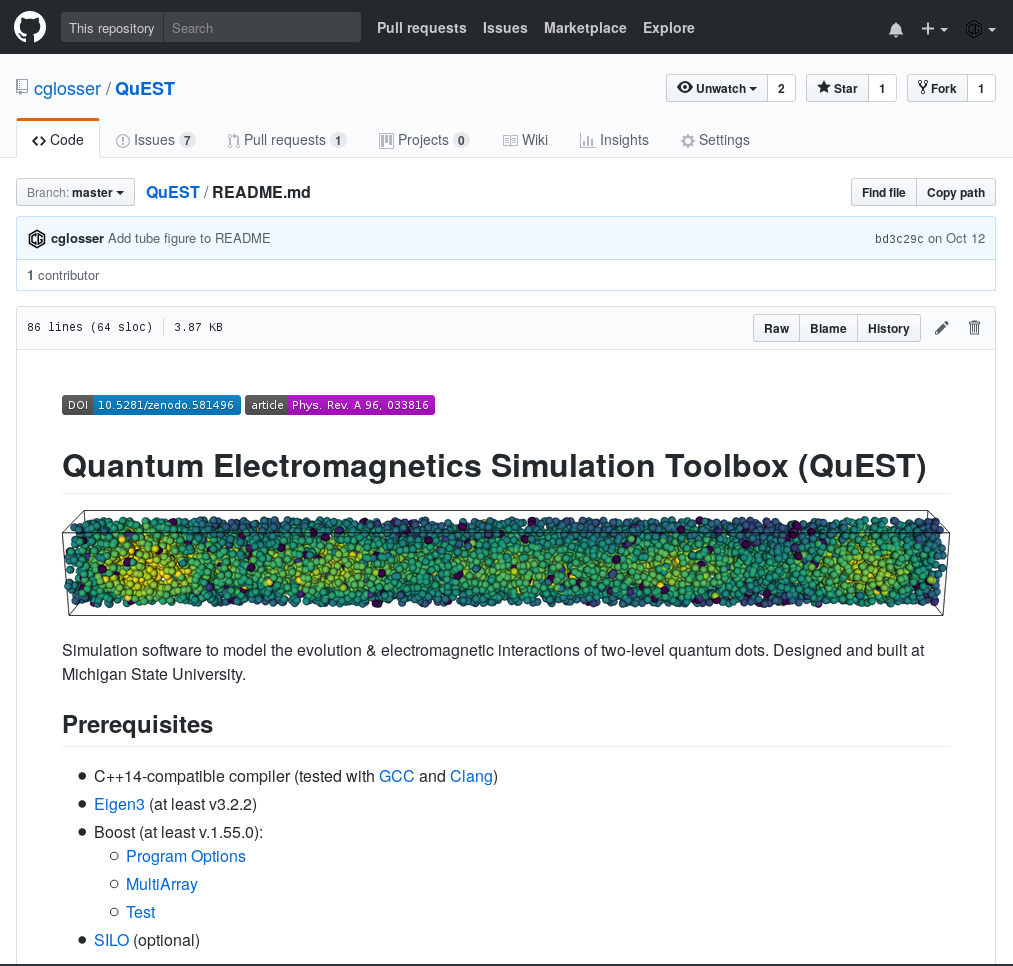
\includegraphics[height=\textheight]{figures/github.png}
\end{frame}

\begin{frame}
  %\begin{center}
    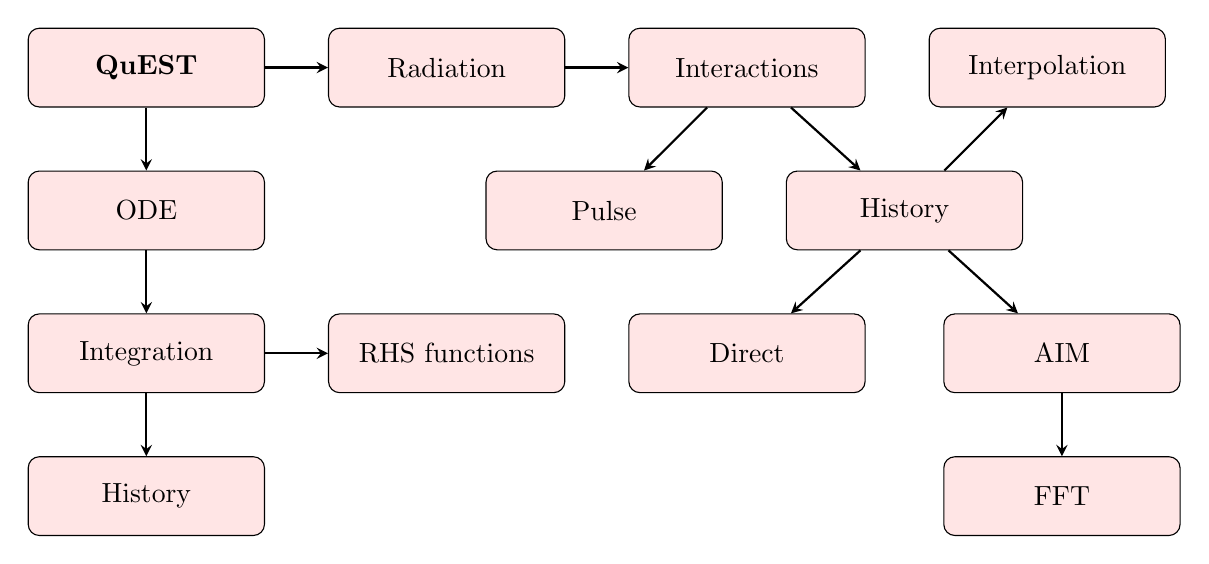
\begin{tikzpicture}[node distance=0.8cm, >=latex]
      \tikzstyle{startstop} = [rectangle, rounded corners, minimum width=3cm, minimum height=1cm,text centered, draw=black, fill=red!10]
      \tikzstyle{io} = [trapezium, trapezium left angle=70, trapezium right angle=110, minimum width=3cm, minimum height=1cm, text centered, draw=black, fill=blue!30]
      \tikzstyle{process} = [rectangle, minimum width=3cm, minimum height=1cm, text centered, draw=black, fill=orange!30]
      \tikzstyle{decision} = [diamond, minimum width=3cm, minimum height=1cm, text centered, draw=black, fill=green!30]
      \tikzstyle{arrow} = [thick,->,>=stealth]

      \node (quest) [startstop] {\textbf{QuEST}};
      \node (ode) [startstop, below= of quest] {ODE};
      \node (radiation) [startstop, right= of quest] {Radiation};

      \draw [arrow] (quest) -- (ode);
      \draw [arrow] (quest) -- (radiation);

      \node (interactions) [startstop, right= of radiation] {Interactions};
      \node (integration) [startstop, below= of ode] {Integration};
      \node (history) [startstop, below= of integration] {History};
      \node (rhs) [startstop, right= of integration] {RHS functions};

      \draw [arrow] (radiation) -- (interactions);
      \draw [arrow] (ode) -- (integration);
      \draw [arrow] (integration) -- (history);
      \draw [arrow] (integration) -- (rhs);

      \node (pulse) [startstop, below= of radiation, xshift=2cm] {Pulse};
      \node (historyI) [startstop, below= of interactions, xshift=2cm] {History};

      \draw [arrow](interactions) -- (pulse);
      \draw [arrow](interactions) -- (historyI);

      \node (interpolation) [startstop, right= of interactions] {Interpolation};
      \node (direct) [startstop, below= of historyI, xshift=-2cm] {Direct};
      \node (aim) [startstop, below= of historyI, xshift=2cm] {AIM};

      \node (fft) [startstop, below= of aim] {FFT};

      \draw [arrow] (historyI) -- (interpolation);
      \draw [arrow] (historyI) -- (direct);
      \draw [arrow] (historyI) -- (aim);
      \draw [arrow] (aim) -- (fft);

    \end{tikzpicture}
  %\end{center}
\end{frame}

\end{document}
